\tikzstyle{arrow_1}=[-->];
\tikzstyle{invisible} = [outer sep=0,inner sep=0,minimum size=0]
\tikzstyle{bordered} = [draw,outer sep=0,inner sep=1,minimum size=10]


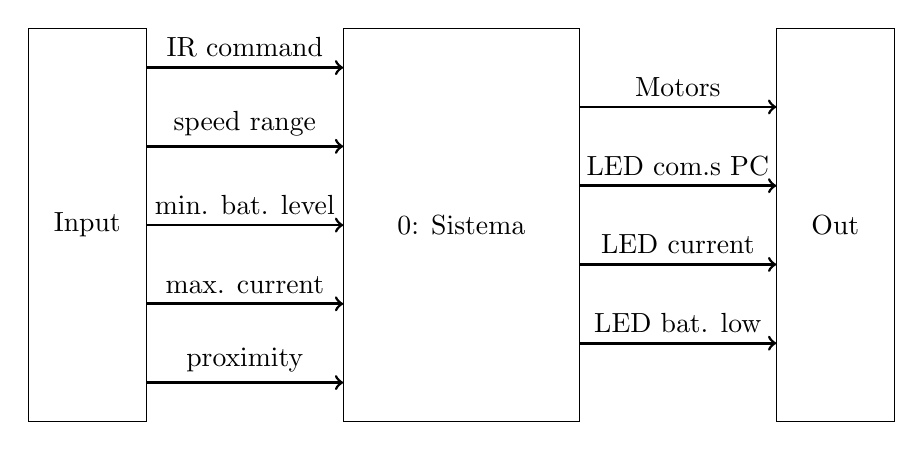
\begin{tikzpicture}

\draw  (-3,4) rectangle (0,-1);
\draw  (2.5,4) rectangle (4,-1);
\draw  (-5.5,4) rectangle (-7,-1);


%INPUT
\node [invisible] (v1) at (-5.5,3.5) {};
\node[invisible]  (v2) at (-3,3.5) {};
\draw[->, draw=black, line width=1pt] (v1) edge  node[midway, auto] {IR command}(v2);

\node [invisible] (v1_1) at (-5.5,2.5) {};
\node [invisible] (v2_1) at (-3,2.5) {};
\draw[->, draw=black, line width=1pt] (v1_1) edge  node[midway, auto] {speed range}(v2_1);

\node [invisible] (v1_2) at (-5.5,1.5) {};
\node [invisible] (v2_2) at (-3,1.5) {};
\draw[->, draw=black, line width=1pt] (v1_2) edge  node[midway, auto] {min. bat. level}(v2_2);

\node [invisible] (v1_3) at (-5.5,0.5) {};
\node [invisible] (v2_3) at (-3,0.5) {};
\draw[->, draw=black, line width=1pt] (v1_3) edge  node[midway, auto] {max. current}(v2_3);

\node [invisible] (v1_4) at (-5.5,-0.5) {};
\node [invisible] (v2_4) at (-3,-0.5) {};
\draw[->, draw=black, line width=1pt] (v1_4) edge  node[midway, auto] {proximity}(v2_4);


% OUTPUT
\node [invisible] (v1) at (0,3) {};
\node[invisible] (v2) at (2.5,3) {};
\draw[->, draw=black, line width=1pt] (v1) edge  node[midway, auto] {Motors}(v2);

\node [invisible] (v1_1) at (0,2) {};
\node [invisible] (v2_1) at (2.5,2) {};
\draw[->, draw=black, line width=1pt] (v1_1) edge  node[midway, auto] {LED com.s PC}(v2_1);

\node [invisible] (v1_2) at (0,1) {};
\node [invisible] (v2_2) at (2.5,1) {};
\draw[->, draw=black, line width=1pt] (v1_2) edge  node[midway, auto] {LED current}(v2_2);

\node [invisible] (v1_3) at (0,0) {};
\node [invisible] (v2_3) at (2.5,0) {};
\draw[->, draw=black, line width=1pt] (v1_3) edge  node[midway, auto] {LED bat. low}(v2_3);

\node at (-1.5,1.5) {0: Sistema};




\node at (-6.25,1.5) {Input};
\node at (3.25,1.5) {Out};
\end{tikzpicture}
     
    